% LaTeX Template for Project Report, Version 2.0
% (Abstracted from a Major Project Report at CSED, NIT Calicut but can be
% modified easily to use for other reports also.)
%
% Released under Creative Commons Attribution license (CC-BY)
% Info: http://creativecommons.org/licenses/by/3.0/
%
% Created by: Kartik Singhal
% BTech CSE Batch of 2009-13
% NIT Calicut
% Contact Info: kartiksinghal@gmail.com
%
% It is advisable to learn the basics of LaTeX before using this template.
% A good resource to start with is http://en.wikibooks.org/wiki/LaTeX/
%
% All template fields are marked with a pair of angular brackets e.g. <title here>
% except for the ones defining citation names in ref.tex.
%
% Empty space after chapter/section/subsection titles can be used to insert text.
%
% Just compile this file using pdflatex after making all required changes.

\documentclass[12pt,a4paper]{report}
\usepackage[pdftex]{graphicx} %for embedding images
\usepackage{algorithm}
\usepackage{algorithmic}
\usepackage{url} %for proper url entries
\usepackage[bookmarks, colorlinks=false, pdfborder={0 0 0}, pdftitle={An Experimental Compiler Design Platform}, pdfauthor={Nachiappan V.}, pdfsubject={<subject here>}, pdfkeywords={<keywords here>}]{hyperref} %for creating links in the pdf version and other additional pdf attributes, no effect on the printed document
%\usepackage[final]{pdfpages} %for embedding another pdf, remove if not required

\begin{document}
\renewcommand\bibname{References} %Renames "Bibliography" to "References" on ref page

%include other pages
\begin{titlepage}

\begin{center}

\textup{\small {\bf CS 4098 Project} \\ Report}\\[0.2in]

% Title
\Large \textbf {An Experimental Compiler Design Platform}\\[0.5in]

       

       {\bf Interim project report}\\[0.5in]

% Submitted by
\normalsize Submitted by \\
\begin{table}[h]
\centering
\begin{tabular}{lr}\hline \\
Roll No & Names of Students \\ \\ \hline
\\
B100168CS & Arun Rajan \\
B100780CS & Nachiappan V. \\ \\ \hline 
\end{tabular}
\end{table}

\vspace{.1in}
Under the guidance of\\
{\textbf{Dr. Murali Krishnan K}}\\[0.2in]

\vfill

% Bottom of the page
\includegraphics[width=0.18\textwidth]{./nitc-logo}\\[0.1in]
\Large{Department of Computer Science and Engineering}\\
\normalsize
\textsc{National Institute of Technology Calicut}\\
Calicut, Kerala, India -- 673 601 \\
\vspace{0.2cm}
Winter Semester 2014

\end{center}

\end{titlepage}

\vspace{2in}
\begin{abstract}
This project proposes a new educational platform for compiler design as an improvisation of the currently existing framework being used at the compiler construction laboratory in our institution. This involves building a compiler for a simple but a non-trivial programming language. We have designed the platform in such a manner that the students would build the compiler in a simple yet systematic method. The process has been broken down into smaller components and implemented stage by stage. Even though this has already been done in theory as well as practice, in our opinion, the correlation between them often goes unnoticed. The different stages have been integrated in such a way that their interlinking is given a lot of importance. This project is aimed at developing a self-sufficient experimental compiler design platform where students can build their own compiler with minimal expert supervision.
\end{abstract} 


\pagenumbering{roman} %numbering before main content starts
\tableofcontents

\newpage
\pagenumbering{arabic} %reset numbering to normal for the main content
\cleardoublepage
%\pagebreak
\phantomsection
\addcontentsline{toc}{chapter}{Acknowledgements}
\chapter*{Acknowledgments}
\vspace{1.0in}
We take extreme pleasure in expressing our deep sense of gratitude to our project guide Dr. Murali Krishnan K., Associate Professor, CSED, NIT Calicut. We are greatly indebted for his guidance and all the required facilities he has provided us during the project.

We would like to express our sincere thanks to our project coordinators Mr. Gopakumar (Assistant professor, CSED, NITC) and Mr.Jayaraj P.B (Assistant professor, CSED, NITC) for having provided us with such wonderful advise.
  
We would be grateful forever to Shamil C.M. for providing us a strong insight into the development of the online platform which is a crucial part of the project.

We would like to express our gratitude to Mevin Dominic and Peeyush Singh for helping us with minor technical contributions. 

Special thanks to colleagues, friends and seniors who have been extremely supportive through out the project.  
{National Institute of Technology Calicut}\\
\newpage %objective changed to problem definition
\chapter{Problem Definition}


Compiler design involves a series of stages of development. Currently, an incremental approach is being used in building a compiler in the compiler construction laboratory in our institution. In this methodology, students are trained to develop a compiler for the Simple Integer Language (SIL). Students are expected to develop a compiler to translate the source code of SIL into executable code which is executed using the Simple Integer Machine (SIM). SIL is an experimental programming language which was designed for educational purposes \cite{citation-3-name-here} and SIM is a virtual machine with an elementary instruction set\cite{citation-4-name-here}. The language chosen for implementing the compiler is the C programming language. Compiler generation tools LEX and YACC have been used to aid the students to build the compiler. 
\\ 
\\
In this currently used approach, we found that many students who enrolled for the compiler laboratory course (including ourselves) faced problems with correlating the compiler design theory with the implementation process. In our opinion, the students would be able to comprehend the process better with more educational resources and guidance. 
\\
\\
Our project attempts to improvise the currently existing system by designing a new instructional framework consisting of documentation for the compiler construction process and an easy to follow roadmap to guide a student who is in the learning phase.    %objective changed to problem definition
\chapter{Introduction}

This project aims to develop an online self-sufficient educational platform which can be used to tutor students in writing a compiler. The project will provide the students with a roadmap for the development process and guide them along the roadmap with supporting documentation. Using the step-by-step guidance offered by the roadmap, the students will be able to build the compiler under minimal expert supervision.
\\
\\
We have designed the platform assuming that a student before starting to follow the roadmap has a basic knowledge of Data structures, Computer organization and a working proficiency of the C programming language. Being instructional in nature, this project gives the learner an insight into the working of LEX, YACC and the usage of these tools to develop a compiler for SIL (Simple Integer language). The theory involved would be learned on a \textit{need-to-do} basis. This, in our opinion would further enhance the understanding of the theory behind the implementation process.
\\
\\
An \textit{in-depth} explanation approach of the compiler design concepts and how these are interlinked with the back-end working of the compiler-generation tools has been used throughout the documentation. We believe that this would enable the students to have a better comprehension of the construction process and the convoluted nature of the different stages of construction. 
\\
\\
The primary focus of the project is to make the compiler construction process an easier task than it currently is now at the laboratory and to provide a strong foundation of basic knowledge in compiler development. %literature survey included in this
\chapter{Literature review}
\section{Compilation process review}
A compiler translates a given source program in a specific programming language into executable code\cite{citation-2-name-here}. The executable code generated is dependent on the machine architecture on which the compiler is being built upon. A simple compiler (without any code optimizer) consist of five phases: Lexical Analysis, Syntax Analysis, Semantic Analysis, Intermediate code generation and Code generation (machine architecture specific)\cite{citation-1-name-here}. The first two phases are the initial focus of the project and are discussed below. 
\section{Lexical analysis using LEX}
Lexical analysis is the process of breaking up a source program into tokens. A lexical token is a sequence of characters that can be treated as a unit in the grammar of a programming language \cite{citation-1-name-here}. A lexical analyzer scans a given input and produces an output of tokens.

LEX is a tool that translates a set of regular expression specifications into a C implementation of a corresponding finite state machine\cite{citation-1-name-here}. This C program when compiled, yields an executable lexical analyzer. Conceptually, LEX constructs a finite state machine to recognize all the regular expression patterns specified in the LEX program file. The lex.yy.c program stores information about the finite state machine in the form of a decision table (transition table). LEX makes it's decision table visible if we compile the LEX program with the \texttt{-T} flag. The finite state machine used by LEX is a deterministic finite state automaton (DFA). The lex.yy.c file simulates the DFA.

Also, LEX offers features to execute a single or compound C statement when a pattern match is found in the input stream. Given its ability to scan and identify a given pattern, and the ability to execute a corresponding action, LEX can be used to generate a lexical analyzer.
 
\section{Syntax analysis using YACC}
Syntax analysis follows lexical analysis in the compilation process. The syntax of a programming language can be expressed using Context Free Grammars (CFG). Any sentential form of the programming language's grammar is considered a syntactically correct program. The process of checking whether a program can be derived from the programming language's grammar is referred to as \textit{parsing}. 
YACC (Yet Another Compiler Compiler) was developed in 1970 by Stephen C. Johnson at AT\& T  Corporation. YACC is a tool that translates the given CFG specification in a YACC program to a corresponding Push Down Automaton (PDA) implementation in C language. The generated C program when compiled, yields an executable parser. The source program is fed to the parser to check if it is syntactically correct.
 
\section{Semantic analysis using YACC}
In addition to syntax analysis, YACC also provides features to support semantic analysis of the source program. Semantic analysis is achieved using C code. C code can be extensively embedded into a YACC program. YACC provides support for add an action to be executed with every grammar rule. These actions are written in C. To support the C code in the actions section, YACC provides an auxiliary functions section (also written in C).

\chapter{Design}

This chapter contains the proposed design which has been followed up till the current state of the project and will be followed (or improvised upon) in later developments of the project if any.

\section{Documentation}

This project will consist of vast amount of documentation on the usage of LEX and YACC to generate a compiler. Initially, the documentation phase will concentrate more on the mastery of the tools and gradually introduce compiler design concepts and how these can be implemented using these tools. The first four stages of the documentation have been designed and compiled successfully. More details of which can be noted in the "Current status" section. 

The documentation follows a very simple explanation approach using plenty of examples and input/output samples. The documentation has been extensively embedded with URLs which link to external or internal resources and references. The idea is to reduce the amount of time a learner spends in the beginning stages and instead invest this time in later on stages of compiler construction which are comparatively more complex. This way, the learner will be able to spend more time in implementing challenging compiler patches instead of spending a lot of time in the learning phase.

\section{Testing}

The document has been embedded with plenty of code in examples and exercises. Before being used in the documentation, each and every code snippet has been implemented and tested in the laboratory. 

\section{Source Language}

This project involves developing a compiler for a source language. Even though the project is still in it's early phases of compiler development, it proposes a source language using which the later stages of the project can be developed.  SIL\cite{citation-3-name-here} is the chosen source language. As a part of the project, a few extensions have been provided to the existing language specification of SIL. These extensions could play a vital role in the learning process.
 
\section{Roadmap}

The Road map is the key to the achieving the project's objective. Along with the documentation and given code snippets, a learner would be asked to follow the roadmap. This project provides the the first four stages of the roadmap.
 
\section{Version Control}
Since this project contains various components and evolves through many stages, it needs to be maintained using a version control system. The advantage of using one would be the ease of  being able to roll back to any version at any point of time during the development phase of the project. We have chosen Git for this purpose.

\section{Online platform}
To enhance the availability of the project to students, this project will be hosted online at the public domain \textbf{silcnitc.github.io}. The website is being developed with HTML5, CSS3 and JavaScript. Github is a remote server for Git. Under licensed conditions, the project will be released on an open source basis on Github. 

\section{Assembling the framework}
Students will use the roadmap to build a compiler for SIL. Towards the code generation phase, they would be instructed to generate code for the SIM architecture\cite{citation-4-name-here}. Once all the individual components have been completely developed, they will be tested and/or proof read several times before they will be integrated with each other appropriately on the website.
\chapter{Current status}
With the current work progress, the platform can be potentially deployed for tutoring a learner with the compiler development tools and basic concepts of compiler development including lexical analysis and syntax analysis. The exact details of the stages are as follows: 
\section{LEX Documentation}
A LEX document for the lexical analysis phase has been designed, compiled and reviewed. 
\section{YACC Documentation}
A YACC document for the syntax analysis phase has been designed, compiled and reviewed.
\section{LEX-YACC Documentation}
A LEX-YACC document for using YACC effectively with LEX has been designed, compiled and reviewed.
\section{Attributes Documentation}
A document on using the attribute stack of YACC has been designed, compiled and reviewed.  
\section{Extensions to SIL}
SIL is a strictly typed language with support for integer and boolean types alone. Currently does not provide support for user-defined types. In this section, we have proposed a language construct called "newtype" which can be used to create user defined data types in SIL.

"newtype" is a new language construct which can be used in the below shown syntax:
\begin{verbatim}
newtype
	typename
	{
		datatype variable_name;
		datatype variable_name;
	}
endtype			
\end{verbatim}
Each new user defined type can have upto a maximum of 8 variables which are either of a built-in data type or or a already defined user-defined data type. The syntax rules and the evaluation rules of the language construct have been provided in the "Appendix". 

The new types will be stored in a data structure similar to the symbol table, called the Type table. A sample type table looks like this:
\linebreak
\begin{center}
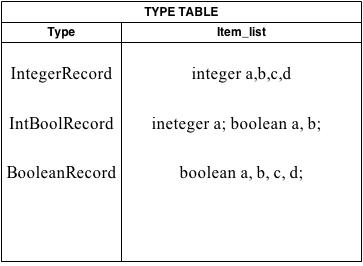
\includegraphics[width=0.4\textwidth]{./type_table.jpg}\\[1in]
\end{center}


\section{Online Platform}
The development of the mainframe of the website has been completed. All the completed documents are available online. Other components of the website are currently under construction. 

\chapter{APPENDIX}
\section{Syntax rules for "newtype"}
The syntax for the "newtype" construct has been provided below. We have used the YACC rules specification to express the syntax.

\begin{verbatim}
%token NEWTYPE VAR INTEGER BOLEAN

%%
typedef			: NEWTYPE typename '{' declaration_list '}' ENDTYPE
				;

declaration_list: declaration_list declaration
				| declaration
				;

declaration		: typename list_var ';'
				;

list_var		: list_var ',' VAR	
				| VAR				
				;

typename		: INTEGER
				|	BOOLEAN
				| VAR   
				;
				
%%
\end{verbatim}

\section{Evaluation rules for "newtype"}
The evaluation rules for the "newtype" construct has been provided below. We have used the YACC rules specification to express the semantics.

\begin{verbatim}
%{

/* Every item-list in the type table*/
struct table_entry
{
	char* id_name;							/* name of variable */
	char* type;								/* data type of variable */
	int binding;							/* address of the variable in memory*/	
	struct table_entry *next;				/* pointer to next entry */
};

/* Every type entry in the type table */
struct type_table
{
	char* type;
	struct table_entry *item_list;
};

/* Head pointer of the type table*/
struct type_table *HEAD;

/*Function to add an item list to the type table */
void add_type (char* type, struct table_entry *item_list);

/*Function to add an item entity to the end of an item list */
struct table_entry *append (struct table_entry *item_list, struct table_entry *item_entity);

/* Fuction to make an item which can be added to the item list */
struct table_entry *list_entity (char *type, char *id_name);

/* Function which returns the number of items in an item list*/
int list_len (struct table_entry *item_list);

/* Function to flag an error */
void yyerror(char *s);

%}

%union{
	char *type;
	struct table_entry *tentry;			
}

%token NEWTYPE 
%token <type> VAR INTEGER BOLEAN 

%type <tentry> id list_var declaration declaration_list 
%type <type> typename
%%

typedef: NEWTYPE typename '{' declaration_list '}' ENDTYPE			
																										{ 	if(list_len($4)<=8)
																													if(!existing_type(typename))
																														add_type(typename, $4);
																													else
																														yyerror("type already exists");
																												else
																														yyerror("type contains too many items");		
																										} 
			;

declaration_list: declaration_list declaration    	{ $$ = append($1,$2); }
				| declaration						{ $$ = $1; }				
	;

declaration: typename { $<type>$=$1;} list_var ';'	{ $$ = $3; }
			;

list_var: list_var ',' {$<type>$=$<type>0;} id			{ $$ = append($1,$4); }
		| {$<type>$=$<type>0;} id						{ $$ = $1; }		
		;

id: VAR									{	$$ = list_entity($<type>0,$1); }
	;

typename: 	INTEGER						{ $$ = $1; }
		| BOOLEAN						{ $$ = $1; }
		| VAR  							{ $$ = $1; } 
				;

%%
/* Auxiliary function definitions */
\end{verbatim}
\input{./ref.tex}

\end{document}
